\documentclass[letterpaper,10pt]{article}
%paquetes
\usepackage[spanish, es-noquoting]{babel}%formato de las tablas
\usepackage[utf8]{inputenc}
\usepackage{enumerate}
\usepackage{graphicx}
\usepackage{float}
\usepackage[T3,T1]{fontenc}
\usepackage{amsmath,wasysym,amssymb,amsfonts,textcomp,latexsym}
\usepackage{hyperref}
\usepackage{appendix}
\usepackage{enumitem}
\usepackage[ruled,vlined,lined,linesnumbered,algosection,spanish]{algorithm2e}
\usepackage{multimedia}
%\usepackage[intlimits]{amsmath}
\usepackage{flexisym}
\usepackage{xparse}
\usepackage{mathtools}
\usepackage{bm}
%\usepackage{draftwatermark}

%\SetWatermarkText{\textsc{Borrador}}
%\SetWatermarkScale{5}
%\SetWatermarkAngle{55}
%%%
% \usepackage{ragged2e}
% \usepackage{pstricks,enumerate}

%\setpapersize{A4}
% Numeración
%\usepackage{vmargin}
%\setmargins{1.5cm}       % margen izquierdo
%{1.5cm}                        % margen superior
%{16.5cm}                      % anchura del texto
%{23.42cm}                    % altura del texto
%{10pt}                           % altura de los encabezados
%{1cm}                           % espacio entre el texto y los encabezados
%{0pt}                             % altura del pie de página
%{2cm}                           % espacio entre el texto y el pie de página
\setcounter{secnumdepth}{30}
\title{Propuesta Alberto Rodríguez Sánchez}

\begin{document}
\renewcommand{\refname}{Bibliografía}.
% Página sin estilo para portada quitar encabezado, pie y número de página
\thispagestyle{empty}

\begin{center}
    {\Huge Universidad Autónoma Metropolitana }\\
    {\huge Unidad Azcapotzalco}\\
    \vspace{0.5cm}
    {\Large División de Ciencias Básicas e Ingeniería}\\
    \vspace{1.0cm}
    {\large Posgrado en Optimización}\\
    \vspace{2.0cm}    
    {\Large TODO}\\
    \vspace{1.0cm}
    {\large Propuesta de Proyecto de Investigación}\\
    \vspace{2.0cm}
    {\large\textbf{Alumno:}}\\
    Alberto Rodríguez Sánchez\\
    %\bigskip 2153800510\\
    \vspace{1.5cm}
    \bigskip
    {\large\textbf{Asesores:}}\\
    Dr. Antonin Ponsich\\
    
    \vspace{1.5cm}
     2017\\
    \vspace{1.0cm}
    Ciudad de México\\
\end{center}
\newpage
\tableofcontents
\newpage
\section{Introducción}

El problema de optimización multiobjetivo \textbf{(MOP)} ha sido de gran interés en la comunidad científica e industrial, ya que son comunes aquellos problemas que requieren
considerar múltiples objetivos incluyendo tiempo, costos, cantidad, calidad, etc. Estos objetivos se encuentran típicamente en conflicto y se pueden encontrar inmersos en
diferentes problemas como: ruteo de vehículos, localización, cadenas de suministro, calendarización, entre otros.\\

Si esta clase de problemas ha sido tradicionalmente atacada reduciendo el \textbf{MOP} en un problema mono-objetivo (estrategia de suma agregativa ponderada, de restricciones-$\epsilon$,
de programación por metas), desde los años 1990, los esfuerzos de investigación se han dedicado al desarrollo de técnicas heurísticas, y particularmente Algoritmos Evolutivos (AEs).
Desde el punto vista metaheurístico se han generado tres grandes enfoques para resolver el \emph{MOP}:

\begin{itemize}
 \item Basado en descomposición
 \item Basado en dominancia
 \item Basado en métricas
\end{itemize}

El enfoque de descomposición explícitamente descompone un problema multiobjetivo en $N$ problemas de optimización escalar y suele introducir técnicas poblacionales para
la resolución simultánea de ellos. Bajo este enfoque, es importante seleccionar los problemas escalares conforme a algún criterio que permita mejorar la diversidad del conjunto
de soluciones arrojado, dejando la convergencia al sub-método de resolución. Un marco de trabajo moderno con este enfoque es el algoritmo evolutivo multiobjetivo basado en
descomposición (\emph{MOEA/D})\cite{4358754}.
\newline

En el enfoque de dominancia, se utilizan las relaciones de dominancia para inducir un orden parcial en el espacio de los objetivos y, de esta manera, decidir cuándo una solución
en dicho espacio es comparable con otra y, en este caso, cuál es la mejor. Cabe mencionar que dicho orden parcial está limitado en espacios de altas dimensiones puesto que una gran
cantidad de soluciones serán no comparables, mermando en consecuencia la efectividad de los procedimientos de selección. El algoritmo genético de ordenamiento no dominado
(\emph{NSGA-III})\cite{6600851} es un marco de trabajo moderno con esta estrategia, que incorpora además técnicas de nichos para mantener la diversidad.
\newline

Finalmente, el enfoque basado en métricas convierte el problema multiobjetivo original en un problema mono objetivo ó multiobjetivo diferente que optimiza el valor de métricas de desempeño,
representando la calidad del conjunto de soluciones obtenidas tanto en términos de convergencia como de dispersión y uniformidad de su distribución. Una métrica popular
es el hipervolumen ya que es la única acorde a la definición de  optimalidad de Pareto (i.e., las soluciones Pareto-óptimas son aquellas que maximizan el hipervolumen).
Sin embargo, calcular el hipervolumen se vuelve costoso conforme aumenta la dimensión del problema multiobjetivo original, por ejemplo, la mejor forma conocida de calcular
el hipervolumen tiene una complejidad de $O(n^2m^3)$ donde $n$ es el número de soluciones aproximadas y $m$ el número de objetivos.
\newline

Un conjunto de soluciones candidatas entregadas por cualquiera de los enfoques antes mencionados debe de cumplir con criterios de convergencia y diversidad para ser
considerado aceptable. Esta meta de obtener un conjunto de soluciones diversas y uniformemente distribuidas se ve dificultada cuando los métodos de solución deben lidiar con:

\begin{itemize}
 \item Convexidad o no convexidad del frente óptimo de Pareto.
 \item Discontinuidad del frente óptimo de Pareto.
 \item Densidad no uniforme de las soluciones en el frente óptimo de pareto.
\end{itemize}

En general, los enfoques basados en dominancia y descomposición utilizan puntos y/o vectores de referencia, que representan direcciones de búsqueda en el espacio objetivo. Pero si bien se han estudiado distintos métodos para generarlos,
sus valores se mantienen clásicamente fijos durante el transcurso de la ejecución del algoritmo,algoritmo. Por lo tanto, el presente proyecto se propone, en primer lugar, comparar la eficacia de diferentes métodos de generación de dicho puntos/vectores de referencia;
y posteriormente, investigar técnicas que permitan ajustarlos en el transcurso de la búsqueda, con el fin de mejorar la diversidad del conjunto solución final.\\

El resto de la presente propuesta se organiza de la siguiente manera. En una segunda sección, se plantea el problema de optimización multi-objetivo en términos generales.
La tercera sección presenta una breve exposicion de los antecedentes. La cuarta sección expone estado del arte sobre los temas relacionados con este estudio. La quinta sección describe el objetivo general,
una sexta sección enumera los objetivos particulares, La séptima sección presenta la metodología a seguir para alcanzar los objetivos descritos en la secciones 5 y 6,
Finalmente la octava sección incluye un cronograma de trabajo.

 
\section{Planteamiento del problema}

El Problema de Optimización Multiobjetivo \textbf{(MOP)} (llamado también
multicriterio o vectorial) puede definirse como el problema de
encontrar (Osyczka, 1985)\cite{Osyczka1985193}:
\begin{quote}
Un conjunto de vectores de variables de decisión que satisfacen un cierto
conjunto de restricciones y optimice un conjunto de funciones
objetivo. Estas funciones forman una descripción matemática
de los criterios de desempeño que suelen estar en conflicto
unos con otros y que se suelen medir en unidades diferentes.
El término ``optimizar'' en este caso toma pues un significado
diferente al del caso de problemas mono-objetivo.
\end{quote}



\subsection{Formulación Matemática}
El problema de Optimización Multiobjetivo \textbf{(MOP)} se define en su forma general de la siguiente manera:
 
$$\min \overrightarrow{F(\bm{x})} = \left[ f_1(\bm{x}), f_2(\bm{x}) , \dots, f_n(\bm{x}) \right] $$
S.A:
 
$$g_i(\bm{x}) \leq 0, i=1,2,\dots,m$$
$$h_j(\bm{x}) = 0, j=1,2,\dots,p$$
$$\bm{x} \in \Omega \subset \mathbb{R}^n$$

Se busca el conjunto de vectores $\bm{x}=[x_1,x_2,\dots,x_k]^T$ que optimicen la función $\overrightarrow{F}$. Las $g_i$ representa las $m$ restricciones de desigualdad y $h_j$ las $p$ restricciones de igualdad.

\subsubsection{Dominancia}

Se dice de un vector $\overrightarrow{U}= (u_1 ,\dots, u_k )$ que domina a otro $\overrightarrow{V}= (v_1 ,\dots, v_k )$ (denotado $\overrightarrow{U} \preceq \overrightarrow{V}$ ) si y sólo si $\overrightarrow{U}$ es parcialmente menor que $\overrightarrow{V}$ , es decir,
$\forall i \in (1,\dots, k), u_i \leq v_i$ y $\exists i \in (1,\dots, k)$ tal que  $u_i<v_i$.

En el contexto del \textbf{MOP},  $\overrightarrow{U}$ y $\overrightarrow{V}$ se encuentran en el espacio de los objetivos.
 
\subsubsection{Optimalidad de Pareto}

Para un problema multiobjetivo dado $\overrightarrow{f(x)}$, el conjunto de óptimos de Pareto ($P^*$) se define como:
$$P^* = ( x \in \Omega | \not\exists x_0 \in \Omega \; : \; \overrightarrow{f(x_0)} \preceq \overrightarrow{f(x)})$$
 
Los vectores $x \in P^*$ son llamados no dominados. La gráfica de las funciones objetivo cuyos vectores no dominados se encuentran
en el conjunto de óptimos de Pareto se denomina frente de Pareto ($\mathcal{PF}$).
 
 
\subsection{Calidad de un conjunto de soluciones del MOP}
 
Hay al menos tres características que debe cumplir un conjunto de soluciones de un problema multiobjetivo:

\begin{itemize}
 \item Precisión: Se refiere a la convergencia del conjunto de soluciones no dominadas (frente aproximado, denotado como $\mathcal{PF}_{aprox}$).. Evalúa qué tan lejos se encuentra del
frente de Pareto óptimo (o frente de Pareto real, denotado como $\mathcal{PF}_{true}$). Cuando el frente de Pareto no se conoce, se emplea un conjunto de referencia.

 \item Diversidad: Mide la uniformidad de la distribución, es decir, la distancia relativa entre las soluciones encontradas.

 \item Dispersión: Se refiere al rango de valores cubierto.
 
\end{itemize}

Una métrica es una función $I:Z_n \rightarrow \mathbb{R}^+$ cuyo valor permite medir la calidad de uno o mas frentes aproximados $\mathcal{PF}_{aprox}$.Algunas métricas utilizadas comúnmente son:

\begin{itemize}
 \item Distancia generacional: La distancia generacional reporta qué tan lejos, en promedio, se encuentra el frente aproximado, $\mathcal{PF}_{know}$ , del frente óptimo, $\mathcal{PF}_{true}$
 $$\bm{GD}(\mathcal{PF}_{know},\mathcal{PF}_{true})=\frac{(\sum^n_{i=1} d_i^p(\mathcal{PF}_{know},\mathcal{PF}_{true}))^{\frac{1}{p}}}{\|\mathcal{PF}_{know}\|}$$
 
 Donde:
 \begin{itemize}
  \item $d_i$ es la distancia mínima entre el punto $p_i \in PF_{know}$ y $PF_{true}$  
  \item $p$ es el parámetro usualmente usado en 1 o 2.
  \item $PF_{know}$ es frente aproximado por el algoritmo.
 \end{itemize}
 
 
 \item Distancia generacional inversa: La distancia generacional inversa reporta qué tan lejos, en promedio, se encuentra un conjunto de vectores uniformemente distribuidos en el frente óptimo, $\mathcal{PF}_{true}$ , del frente aproximado, $\mathcal{PF}_{know}$
 $$\bm{iGD}(PF_{know},PF_{true})=\frac{\sum^n_{i=1} d_i(PF_{know},PF_{true})}{\|PF_{true}\|}$$
 
 Donde:
 \begin{itemize}
  \item $d_i$ es la distancia mínima entre el punto $p_i \in PF_{know}$ y $PF_{true}$  
  \item $PF_{true}$ es frente real por el algoritmo.
 \end{itemize}

 \item Delta Diversidad: La métrica de diversidad (diversity metric) $\Delta$, mide la extensión de la dispersión lograda por las soluciones no dominadas
 $$\bm{\Delta}(\Omega,E_i)=\frac{\sum^k_{i=1} d(E_i,\Omega) + \sum_{p_i \in \Omega} |d(p_i,\Omega)-\overline{d}|}{\sum^k_{i=1} d(E_i,\Omega) + (|\Omega| - k)\overline{d}}$$
 
 Donde:
 \begin{itemize}
  \item $d(p_i,\Omega)$ es la distancia mínima entre el punto $p_i \in \Omega$ y el resto de los elementos en $\Omega$  
  \item $\overline{d}$ es el promedio de $d(p_i,\Omega)$.
  \item $E$ son los puntos extremos del frente real $PF_{true}$.
 \end{itemize}

 \item Hipervolumen: El hipervolumen mide el área, volumen, o hipervolúmen, encerrado entre los puntos en la aproximación del frente de Pareto, $PF_known$
un punto de referencia, $r$.
 $$\bm{\Delta}(PF_{know},r)=\bigcup^N_{i=1} (v|p^j_i \leq v_j \leq r_j , j = 1, \dots, m) $$
 
\end{itemize}


\section{Antecedentes}

Entre los procedimientos metaheurísticos existen distintos marcos de trabajo enfocados a la optimización multiobjetivo, utilizando distintos métodos para asegurar una buena diversidad,
aquí se exponen brevemente el funcionamiento de los marcos de trabajo MOEA/D y NSGA-III, así como las distintas estrategias tomadas para mejorar la diversidad del frente resultante.

\subsection{Marco de Trabajo MOEA/D}
El \emph{MOEA/D} fue desarrollado por Qingfu Zhang y Hui Li de la Universidad de Essex en 2007. \cite{4358754},

Es un algoritmo de optimización inspirado en las técnicas de descomposición y los algoritmos genéticos. El proceso de descomposición requiere de un conjunto de vectores de peso,
que deben cumplir con estar distribuidos uniformemente en el espacio de las soluciones. Es requerida ademas, una función de escalarización que admita diferentes vectores de peso, en principio,
las funciones de sumas ponderadas  ($g^{ws}$) y pesos de Chebyshev ($g^{te}$) son usadas en la propuesta original del algoritmo y se definen como sigue:

\begin{enumerate}
\item La función de sumas ponderadas define el siguiente problema de optimización escalar:
$$\min g^{ws}(x\|w) = \sum^M_{i=1} w_if_i(x) $$
S.A:
$$ \sum^M_{i=1} w_i = 1$$
$$w \geq 0$$

Esta función suele ofrecer buenos resultados en espacios de soluciones convexos, sin embargo, no es capaz de mapear cada punto del $\mathcal{PF}_{true}$ en espacios no convexos.

\item La función de pesos Chebyshev define el siguiente problema de optimización escalar:

$$\min g^{te}(x\|w) = \max{i=1,\dots,M} w_i(f_i(x) -z^{*})$$

donde:
$$z^{*}= \min (f_i(x) | x \in \Omega) $$

Se ha probado que la función de pesos de Chebyshev puede generar cualquier punto en $\mathcal{PF}_{true}$ sin importar la convexidad del espacio.
\end{enumerate}

Una vez seleccionada la función de escalarización es posible definir $N$ problemas de optimización escalares, la resolución de los problemas se realiza de forma simultánea
por medio de la construcción de un nicho con las soluciones candidatas de los $T$ problemas más cercanos. Este nicho es la población de un algoritmo genético
que mejora las soluciones en cada generación. Como marco de trabajo, \emph{MOEA/D} se distingue por tener las siguientes características:

 \begin{itemize}
 \item Técnicas de análisis geométrico sobre el simplejo del problema \cite{mie99,Das:1998:NIN:588907.589322, Messac2003}
 \item Mejora de soluciones hasta óptimos locales/globales garantizados por el teorema de Holland\cite{Holland:1992:ANA:531075}
 \end{itemize}


\subsubsection{Pseudocódigo MOEA/D}

   \scalebox{.85}{
    \begin{algorithm}[H]
   \caption{Algoritmo MOEA/D}
   %\SetLine
    \KwData{$IterMax$: condición de paro, $N$:subproblemas a considerar, $T$: Tamaño de vecindario, $P_{crossover}$, $P_{mutation}$}
    \KwResult{$PE$:Frente Aproximado}
Poblacion $\leftarrow$ PoblacionInicial($Poblacion_{size}$, $NumObjetivos$)\;
 
$W = {\bm{w}_1,\dots,\bm{w}_N}$ $\leftarrow$ VectoresDePesosUniformementeDistribuidos(N)\;
${B_0,\dots,B_N} \leftarrow$ VecinosCercanos($T$, $W$)\;
 
\While {$\neg$Paro($IterMax$)}{
 
\For {$i:=1$ a $N$}{
Selección $\leftarrow$ SeleccionPadres($B_i$)\;
$C_i$ $\leftarrow$ CruzayMutacion(Selección, $P_{crossover}$, $P_{mutation}$)\;
\If {$C_i \preceq x \in B_i$}{
$x$ $\leftarrow$ $C_i$\;}
}
$PE$ $\leftarrow$ ActualizarPE($Poblacion$)
}
 
\Return($PE$)
\end{algorithm}}

\subsection{Marco de Trabajo NSGA-III}

El marco de trabajo \emph{NSGA-III} fue propuesto por K. Deb and H. Jain en 2014.\cite{6600851}. Utiliza la noción de Golberg sobre ordenamiento no dominado en algoritmos genéticos \cite{goldberg1988genetic}
, es una mejora a NSGA-II para trabajar con problemas de más de $3$ funciones objetivos.

Inicia generando una población padre ($P_t$) de tamaño $N$ en el dominio del problema, utilizando las operaciones de selección, cruza y mutación genera una población descendiente ($Q_t$)
Ambas poblaciones son combinadas y ordenadas en $K$ niveles conforme a los criterios de dominancia (``Non dominated sorting''), los $N$ mejores miembros son seleccionados para formar
la siguiente población padre ($P_{t+1}$), esto es tomando los miembros de los mejores $l-1$ niveles de dominancia. Para completar los $N$ miembros de $P_{t+1}$ es requerido un procedimiento
para seleccionar a los individuos faltantes entre los miembros del nivel $l$. Aquí la diferencia fundamental entre \emph{NSGA-III} y su predecesor es como se realiza la preservación de nichos,
\emph{NSGA-III} propone sustituir ``Crowding distance'' por métodos de nichos de tal manera que ayuden a mejorar la diversidad de la población. Para esto \emph{NSGA-III} genera puntos de referencia
iniciales utilizando en método propuesto por Das \& Dennis en 1998 \cite{Das:1998:NIN:588907.589322} donde se definen $K$ puntos estructurados sobre el simplejo $M$ dimensional.
Para determinar $K$ es requerido $p$ que es un parámetro a ajustar, entonces $K$ puede ser calculada como sigue:
  $$K= {M+p-1 \choose p}$$
Cada punto $\bm{Z}^{(k)}=(z_1^{(k)},z_2^{(k)}, \dots, z_M^{(k)})$ satisface la siguiente condición:
  $$\sum_{i=1}^M z_i^{(K)} = 1$$
Esto generar un hiperplano lineal en $M$ dimensiones con un ángulo igual para cada eje e intersectando cada eje en solo un punto.

\begin{figure}[h]
 \centering
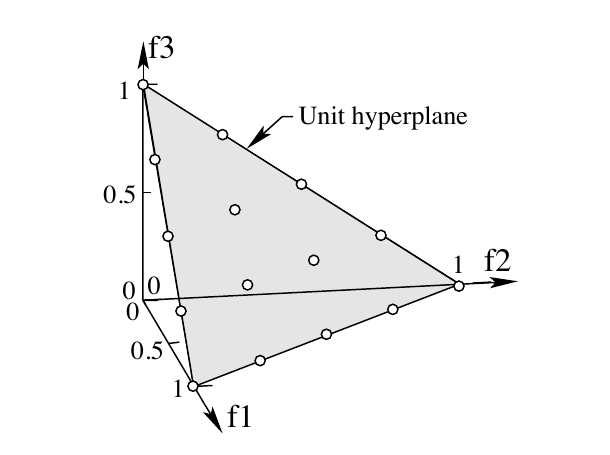
\includegraphics[scale=0.35]{hyper.png}
\caption{Hiperplano unitario generado con el método de Das \& Dennis}.
\end{figure}
Con los puntos de referencia y las magnitudes de las funciones objetivo normalizadas se calcula la distancia ortogonal entre cada punto en nivel $l$ y se asocian a su punto de referencia más cercano,
seguido de un conteo de nichos para seleccionar a los miembros del nivel $l$ en los nichos menos poblados promoviendo la diversidad. Esto se repite hasta cumplir el criterio de paro.


\subsubsection{Pseudocódigo NSGA-III}
 
   \scalebox{.85}{
   \begin{algorithm}[H]
   \caption{Algoritmo NSGA-III}
     
 \KwData{$H$:puntos de referencia estructurados $\bm{Z}^{(s)}$, Poblacion Padre $P_t$}
 \KwResult{$P_{t+1}$}
   $S_t=\emptyset,i=1$\;
   $Q_t = Recombinacion+Mutacion(P_t)$\;
   $R_t = P_t \cup Q_t$\;
   ($F_1,F_2,\dots$) = FastNondominatedSort($R_t$)\;
   
   \Repeat{$|S_t| \geq N$}{
   $S_t = S_t \cup F_i$\;
   $i=i+1$\;
   }
   $F_l = F_i$\;
   \eIf{$|S_t| == N$}{
   $P_{t+1} = S_t$\;
   break\;
   }(\tcc*[f]{Eleccion de los $K$ puntos restantes de $F_l$}){
   $P_{t+1}= \bigcup^{l-1}_{j=1} F_j$\;
   $K=N-\|P_{t+1}\|$\;
   $Normalizar(f^n,S_t,Z^r,Z^s,Z^a)$\;
   $(\pi(s),d(s))=Asociar(S_t,Z^r)$\;
   \For{$j \in Z^r$}{
   $\rho_j =\sum_{s \in S_t \setminus f_l } ( \pi(s) == j )$\;
    }
    $P_{t+1} = Nichos(K,\rho_j,\pi,d,Z^r,F_l, P_{t+1})$\;
   }
   
  \Return ($P_{t+1}$)
\end{algorithm}}

\subsection{Repulsión de subpoblaciones}

En 2016, Ahrari et al. proponen utilizar una técnica de nichos basada en la repulsión de subpoblaciones \cite{ahrari2016multimodal}. Toda subpoblación $P_i$ tiene un tamaño fijo $\lambda$,
sus propios parámetros de cruza y mutación ($\sigma_{mean_i},C_i$), un centro ($x_{mean_i}$) y miembros elite. Existe también un conjunto de puntos prohibidos $y_k$
(mejores soluciones actuales o los centros de las subpoblaciones) que restringen la generación de nuevas soluciones en base a una distancia métrica, es decir, las nuevas soluciones aceptables
se encontraran en regiones poco exploradas del espacio de búsqueda. Una solución se considera aceptable satisface el criterio distancia con todos los puntos prohibidos, de lo contrario,
la solución es rechazada. El efecto general de esta estrategia es una remodelación de las soluciones alcanzadas de tal manera que las subpoblaciones no buscan en regiones del espacio
previamente exploradas y dos subpoblaciones no buscan en la misma región del espacio de búsqueda.
\newline

Esta estrategia de nichos utiliza la distancia de Mahalanobis\cite{mahalanobis1936generalised}, una versión escalada de la distancia euclidiana, permitiendo revisar si una solución esta lo suficientemente
alejada de los puntos prohibidos. La distancia de Mahalanobis ($D_{ij-k}$) de la $j$-ésima solución ($x_{ij}$) de $P_i$, matriz de covarianza $C_i$ y desviación estándar $\sigma_{mean_i}$ al punto prohibido
$y_k$, se define como sigue:

$$D_{ij-k} = \frac{(x_{ij}-y_k)^T C^{-1}_i (x_{ij}-y_k)}{\sigma_{mean_i}}$$

Una consecuencia del uso de esta distancia en particular es que $D_{ij-k}$ es inversamente proporcional a $\sigma_{mean_i}$, es decir, cuando las soluciones convergen $x_{ij}$ a $y_k$,
la distancia $D_{ij-k}$ aumenta. Este comportamiento evita que las nuevas soluciones sean similares a $y_k$.


\subsection{Métodos empleados para resolver el MOP mejorando la diversidad de las soluciones}

Con ambas estrategias (descomposición con el MOEA/D y dominancia con el NSGA-III), la determinación de los vectores de peso o puntos de referencia constituye claramente un factor crítico para obtener una buena diversidad del frente aproximado. Se han propuesto varios algoritmos para generar vectores de pesos iniciales en el caso del enfoque de descomposición como:
\newline


\begin{itemize}
 \item Cheng He \& Linquiang Pan (2016) proponen un método de generación de puntos tomando en cuenta las propiedades de la función objetivo y determinando si la superficie del frente es cóncava, convexa o un hiperplano. Este procedimiento se repite para numerosas subregiones del espacio objetivo, generando experimentalmente un conjunto de puntos mejor distribuido (de acuerdo a la métrica Spacing) que el método de referencia propuesto por de Das y Dennis.\cite{7748353}.    
 \item T. C. Chiang \& Y. P. Lai (2011) consideran dos cambios fundamentales en la estructura de MOEA/D y MOEA/D-DE(en el que la generación de nuevas soluciones candidatas se realiza mediante el operador de mutación de Evolución Diferencial), el primero consiste en crear un criterio de selección del subproblema a resolver si es que éste no se considera resuelto (sin mejora tras cierto número de iteraciones) con el fin de redistribuir el tiempo de cómputo solo en los problemas aún sin resolver. La segunda mejora es la restricción a la cruza aplicada a los individuos en el espacio de las variables de decisión en lugar del espacio de los objetivos. Sin embargo, la generación de los nichos requiere ajustar dos parámetros adicionales que empeoran un proceso de agrupamiento computacionalmente costoso $O(nN^2)$\cite{5949789}.
 \item B. Liu et al. (2010) utilizan una variante de MOEA/D que sustituye al algoritmo genético por evolución diferencial (DE/best/1/bin). Los autores buscan mejorar la diversidad usando un factor de escalamiento aleatorio en la evolución diferencial, además de restringir la cruza al permitir aleatoriamente cruza con individuos fuera de la vecindad. Utilizan descomposición por el método de Tchebycheff \cite{5585957}.
 \item S. Z. Zhao et al. (2010) proponen calcular el tamaño de vecindario en MOEA/D de forma dinámica, generando un ranking de los tamaños que estadísticamente dan mejores resultados. Este proceso se repite recalcula cada cierto número de generaciones, siendo entonces el tamaño de vecindario auto-adaptativo \cite{6151117}.
\end{itemize}

En el caso de el enfoque de dominancia se encontraron los siguientes trabajos:

\begin{itemize}
 \item Haitham Seada \& Kalyanmoy Deb (2015) proponen un algoritmo basado en NSGA-III capaz de adaptarse y funcionar bien en problemas multiobjetivo, mono objetivo y de muchos objetivos ajustando los parámetros del algoritmo según la dimensión \cite{a0ecee762d9f4867a9ded8de598c732e}.
 \item Haitham Seada \& Kalyanmoy Deb (2015) realizan un estudio sobre la restricción del tamaño de población impuesto en el NSGA-III original y proponen una aproximación que solventa esa deficiencia aprovechando las técnicas de nichos \cite{7257251}.
 \item Giagkiozis et al. (2014) introducen el método Cross-entropy (CE) basado en métodos probabilísticos que distribuyen los puntos de referencia acorde a la geometría del frente de Pareto, de tal manera que se maximice el indicador de hipervolumen. CE utiliza métodos poblacionales y reacciona ante eventos para ajustar la distribución de probabilidad y adaptarse al frente \cite{Giagkiozis2014363}.
 \item Himanshu Jain \& Kalyanmoy Deb (2013) desarrollan una distribución adaptativa de los puntos de referencia para asegurar la diversidad, reubicando los puntos referencia que no han sido asociados a soluciones factibles hacia posiciones vecinas donde se espera tengan soluciones asociadas \cite{jain2013improved}.
\end{itemize}

\section{Justificación}

Las metaheurísticas son técnicas de solución versátiles, flexibles y eficientes, estos algoritmos pueden resolver problemas complejos de optimización multiobjetivo \cite{coello1999comprehensive} aproximando el frente real con éxito.
\newline

De esta forma proporcionan un marco de trabajo accesible computacionalmente para encontrar soluciones de buena calidad que además sean diversas, permitiendo a la persona o sistema tomar la decisión adecuada conforme a los criterios que crean pertinentes.
\newline

El presente trabajo adquiere importancia con el estudio de los mecanismos que buscan preservar la diversidad de las soluciones en los principales marcos de trabajo en el estado del arte de \textbf{MOP}, en particular,
la inicialización de vectores de pesos/ puntos de referencia iniciales y la capacidad de adaptar los mismos durante el transcurso de la ejecución de los algoritmos es vital para alcanzar los objetivos de diversidad y convergencia
Tomando como referencia la técnica de repulsión de subpoblaciones proveniente de la optimización multimodal\cite{doi:10.1162/EVCOa00182}, se espera introducir un método de adaptación de puntos de referencia/vectores de pesos que aproveche la información adquirida para redistribuir las referencias para mejorar la diversidad con respecto a alguna métrica.

\section{Objetivo General}

Adaptar e integrar estrategias de generación y actualización de los vectores de peso en el MOEA/D y de los puntos de referencia en el NSGA-III para  evaluar su impacto sobre el desempeño en términos de diversidad de estos dos algoritmos evolutivos multiobjetivo.

\section{Objetivos Particulares}

\begin{itemize}

\item Adaptar, implementar y describir el comportamiento del método \emph{MOEA/D} para las instancias seleccionadas.
 
\item Adaptar, implementar y describir el comportamiento del método \emph{NSGA-III} para las instancias seleccionadas.

\item Adaptar e implementar al menos dos estrategias para generar vectores de peso /puntos de referencia iniciales para \emph{MOEA/D} y \emph{NSGA-III}.

\item Desarrollar al menos una estrategia de actualización de vectores de pesos para el método \emph{MOEA/D}, basada en el método de repulsión de subpoblaciones\cite{ahrari2016multimodal}.

\item Desarrollar al menos una estrategia de actualización de puntos de referencia para el método \emph{NSGA-III}, basada en el método de repulsión de subpoblaciones\cite{ahrari2016multimodal}.

\item Realizar experimentos computacionales sobre un banco de instancias clásicas de optimización multiobjetivo\cite{zhang2008multiobjective} para comparar las diferentes versiones de los algoritmos estudiados, particularmente con respecto a las métricas de diversidad.

\item Realizar experimentos computacionales sobre un banco de instancias clásicas de optimización multiobjetivo\cite{zhang2008multiobjective} para comparar los resultados obtenidos con los reportados en la literatura especializada.  

\end{itemize}


\section{Metodología}

Para la implementación de las dos heurísticas basadas en los enfoques de descomposición y dominancia, se ha estado haciendo una revisión en el estado del arte para analizar las características de los marcos de trabajo NSGA-III y MOEA/D, tomándolas  como  base para la adaptación al problema, posteriormente se propondrán mejoras a estos algoritmos.
 
Posteriormente se realizará un análisis estadístico de cada una de las técnicas implementadas, comparando su rendimiento contra algunas de las  técnicas propuestas en la literatura.
 
 \begin{itemize}
 \item[•] \textbf{ETAPA 1.} \emph{Se analizó el estado del arte para el MOEA/D y NSGA-III identificando los aportes recientes en cuestiones de diversidad.}
\item[] Identificando y listando las técnicas reportadas en tres clases: métodos basados en descomposición, métodos basados en dominancia y métodos basados en métricas. Así mismo, se han revisado las técnicas que se busca implementar al problema analizando su estructura y características.
\emph{(Concluida)}

\item[•] \textbf{Etapa 2.} \emph{Adaptación e implementación de los marcos de trabajo MOEA/D y NSGA-III para incluir mejoras en la selección de vectores/puntos de referencia iniciales y técnicas de adaptación dinámica de los mismos.}

\item[] Con base al análisis del perfil de nuestras técnicas, se implementarán en un lenguaje de programación.
        
\item[•] \textbf{Etapa 3.} \emph{Comparaciones de las técnicas y análisis estadístico.}

\item [] Una vez que se tengan las estrategias implementadas, se realizarán comparaciones de calidad de las soluciones obtenidas por cada una y la cantidad de recursos computacionales  que utilizan. Posteriormente, se justificará su rendimiento con un análisis estadístico detallado para cada  una de estas.

\item[•] \textbf{Etapa 4.} \emph{Proceso de mejora de las técnicas.}

\item[] Las técnicas se someterán a un estudio para identificar si algunas funciones se pueden mejorar con algún cambio en la implementación, que dé como resultado disminución en el tiempo de ejecución o reducción en el costos de recursos.


\item[•] \textbf{Etapa 5.} Comparación de las técnicas definidas y reporte de resultados.

\item[] Una vez terminada la etapa de mejoras de cada una de las técnicas, se realizará un nuevo análisis estadístico para comparar el rendimiento de cada una de nuestra técnicas, describiendo los resultados obtenidos.
        
  \end{itemize}

\subsection{\textbf{Diseño de experimentos}}
Los experimentos consistirán en la medición de la calidad de las soluciones dadas por cada una de las técnicas así como de su tiempo de ejecución para un conjunto de instancias benchmark.
         
\section{Cronograma}
\begin{table}[H]
\centering

\label{tablaTiempos}
\scalebox{0.9}{\begin{tabular}{|l|c|c|c|c|}
\hline
\begin{tabular}[c]{@{}c@{}}Nombre\\   de la tarea\end{tabular} & Fecha de Inicio & Fecha final & \% Completado & Duración \\ \hline
Presentación propuesta de tesis                                & XX/XX/17        & XX/XX/17    & XXX\%         & XXd      \\ \hline
Adaptación MOEA/D con adaptación de vectores                   & XX/XX/17        & XX/XX/17    & XX\%          & XXd     \\ \hline
Adaptación NSGA-III con adaptación de puntos de referencia     & XX/XX/17        & XX/XX/17    &               & XXd      \\ \hline
Análisis y comparación de técnicas                             & XX/XX/17        & XX/XX/17    &               & XXd      \\ \hline
Redacción de tesis                                             & XX/XX/17        & XX/XX/17    &               & XXd      \\ \hline
Entrega de tesis                                               & XX/XX/17        & XX/XX/17    &               & 1d       \\ \hline
\end{tabular}
}
\caption{Cronograma}
\end{table}



% \begin{table}[H]
% \centering
% \label{miOtraTabla}
% \scalebox{0.6}{\begin{tabular}{|l|l|}
% \hline
% Nombre de la tarea                 & \multicolumn{1}{c|}{Metas alcanzar al terminar la tarea}                                                                                                                                                                                                                                                                                                                                                            \\ \hline
% Presentación propuesta de tesis    & Aprobación de propuesta de tesis por el comité de posgrado.                                                                                                                                                                                                                                                                                                                                                         \\ \hline
% Correcciones propuesta de tesis    & Registro de Aceptación de tesis.                                                                                                                                                                                                                                                                                                                                                                                    \\ \hline
% Adaptación FA para el PAG          & \begin{tabular}[c]{@{}l@{}}Se busca describir el comportamiento de la técnica implementada al PAG y probada\\ con algunas instancias disponibles, esperando tener buenos resultados con respecto de\\  las técnicas existentes en la literatura,  comparando la calidad de la solución y el número\\  de llamadas a la función objetivo;  así como las ventajas y desventajas que ofrece esta técnica.\end{tabular} \\ \hline
% Adaptación GSA para el PAG         & \begin{tabular}[c]{@{}l@{}}Se busca describir el comportamiento de la técnica implementada al PAG  y probada \\ con algunas instancias disponibles,  esperando tener buenos resultados con respecto de\\ las técnicas existentes en la literatura, comparando la calidad de la solución y el número\\ de llamadas a la función objetivo; así como las ventajas y desventajas que ofrece esta técnica.\end{tabular}  \\ \hline
% Adaptación MMC para el PAG         & \begin{tabular}[c]{@{}l@{}}Se busca describir el comportamiento de la técnica implementada al PAG y probada \\ con algunas instancias disponibles, esperando tener buenos resultados con respecto de \\ las técnicas existentes en la literatura, comparando la calidad de la solución y el número\\ de llamadas a la función objetivo;  así como las ventajas y desventajas que ofrece esta técnica.\end{tabular}  \\ \hline
% Anélisis y comparación de técnicas & \begin{tabular}[c]{@{}l@{}}Se busca describir el comportamiento de nuestras técnicas con la finalidad de poder\\ decir cuales son sus ventajas o defectos al ser utilizadas con las instancias seleccionadas\\ para el PAG.\end{tabular}                                                                                                                                                                            \\ \hline
% Redacción de tesis                 & Documentación de la investigación realizada.                                                                                                                                                                                                                                                                                                                                                                        \\ \hline
% Entrega de tesis                   & \begin{tabular}[c]{@{}l@{}}Obtener la\\   aprobación y fecha para el examen de grado\end{tabular}                                                                                                                                                                                                                                                                                                                   \\ \hline
% \end{tabular}
% }
% \caption{Metas}
% \end{table}

%\begin{figure}[H]
%\begin{center}
    %\scalebox{0.800}{\includegraphics{cronogramatesis.jpg}}%%%%%%%%%%%%%%%%%%Cambiar imagen.
 
 % \label{sol}
%   \caption{Cronograma.}
   
%\end{center}
%\end{figure}

%\begin{figure}[H]
%\begin{center}
%    \scalebox{0.600}{\includegraphics{cronograma2.jpg}}%%%%%%%%%%%%%%%%%%Cambiar imagen.
 
 % \label{sol}
  % \caption{Cronograma2.}
   
%\end{center}
%\end{figure}
\bibliographystyle{acm}
\bibliography{bibliografia}
\end{document}